\section{Introducción}
\subsection{Evolución de la Concurrencia en Java}
\begin{frame}
    \begin{center}
        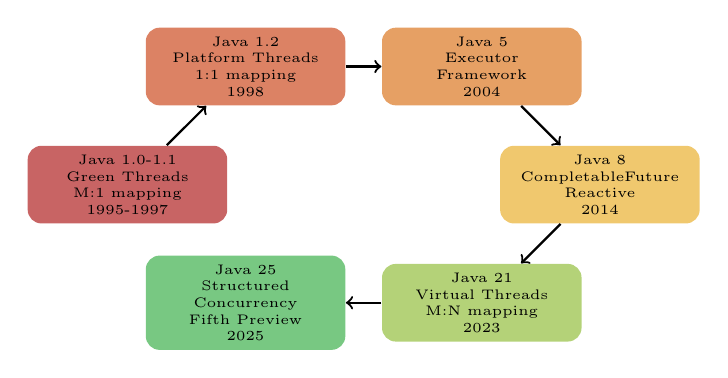
\begin{tikzpicture}[
            box/.style={rectangle, text width=2.3cm, align=center,
            font=\tiny, rounded corners=5pt},
            box1/.style={box, fill={rgb,255: red,200; green,100; blue,100}},
            box2/.style={box, fill={rgb,255: red,220; green,130; blue,100}},
            box3/.style={box, fill={rgb,255: red,230; green,160; blue,100}},
            box4/.style={box, fill={rgb,255: red,240; green,200; blue,110}},
            box5/.style={box, fill={rgb,255: red,180; green,210; blue,120}},
            box6/.style={box, fill={rgb,255: red,120; green,200; blue,130}}
        ]
            \node (green) [box1] at (-3, 0) {Java 1.0-1.1\\Green Threads\\M:1 mapping\\1995-1997};
            \node (platform) [box2] at (-1.5, 1.5) {Java 1.2\\Platform Threads\\1:1 mapping\\1998};
            \node (executor) [box3] at (1.5, 1.5) {Java 5\\Executor\\Framework\\2004};
            \node (reactive) [box4] at (3, 0) {Java 8\\CompletableFuture\\Reactive\\2014};
            \node (virtual) [box5] at (1.5, -1.5) {Java 21\\Virtual Threads\\M:N mapping\\2023};
            \node (structured) [box6] at (-1.5, -1.5) {Java 25\\Structured Concurrency\\Fifth Preview\\2025};

            \draw [->, thick] (green) -- (platform);
            \draw [->, thick] (platform) -- (executor);
            \draw [->, thick] (executor) -- (reactive);
            \draw [->, thick] (reactive) -- (virtual);
            \draw [->, thick] (virtual) -- (structured);
        \end{tikzpicture}
    \end{center}
    \begin{alertblock}{Estado en Java 25}
        \begin{itemize}
            \item Virtual Threads: \textbf{Estable} (desde Java 21)
            \item Scoped Values: \textbf{Estable} desde Java 25 ~\cite{JEP506}
            \item Structured Concurrency: \textbf{Quinta Preview} en Java 25 ~\cite{JEP505}
        \end{itemize}
    \end{alertblock}
\end{frame}
\subsection{Problema de ejemplo: Procesamiento de Transacción Financiera}
\begin{frame}
    \frametitle{Flujo ficticio}
    \begin{center}

        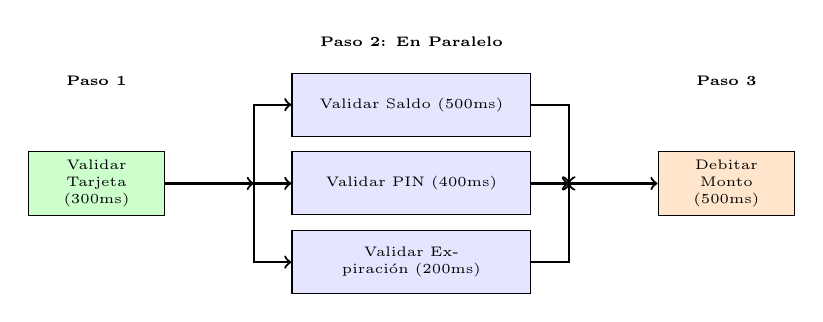
\begin{tikzpicture}[
            node/.style={draw, rectangle, text width=1.5cm, align=center, font=\tiny, minimum height=0.8cm},
            parallel/.style={draw, rectangle, text width=2.8cm, align=center, font=\tiny, fill=blue!10, minimum height=0.8cm},
            arrow/.style={->, thick}
        ]

% Nodes positioned manually for precise alignment
            \node (card) [node, fill=green!20] at (0,0) {Validar \\ Tarjeta \\ (300ms)};

% Parallel validations - perfectly aligned vertically
            \node (balance) [parallel] at (4,1) {Validar Saldo (500ms)};
            \node (pin) [parallel] at (4,0) {Validar PIN (400ms)};
            \node (expiry) [parallel] at (4,-1) {Validar Expiración (200ms)};

            \node (debit) [node, fill=orange!20] at (8,0) {Debitar \\ Monto \\ (500ms)};

% Coordination points for line division and convergence
            \coordinate (split) at (2,0);
            \coordinate (join) at (6,0);

% Arrows with structured lines
% From card to split point
            \draw [arrow] (card.east) -- (split);

% From split point to parallel validations (vertical then horizontal)
            \draw [arrow] (split) -- (2,1) -- (balance.west);
            \draw [arrow] (split) -- (pin.west);
            \draw [arrow] (split) -- (2,-1) -- (expiry.west);

% From parallel validations to join point (horizontal then vertical)
            \draw [arrow] (balance.east) -- (6,1) -- (join);
            \draw [arrow] (pin.east) -- (join);
            \draw [arrow] (expiry.east) -- (6,-1) -- (join);

% From join point to debit
            \draw [arrow] (join) -- (debit.west);

% Labels
            \node [above of=card, yshift=0.3cm, font=\tiny]{\textbf{Paso 1}};
            \node [above of=pin, yshift=0.8cm, font=\tiny] {\textbf{Paso 2: En Paralelo}};
            \node [above of=debit, yshift=0.3cm, font=\tiny]{\textbf{Paso 3}};

        \end{tikzpicture}
    \end{center}

    \begin{alertblock}{Flujo Optimizado}
        \textbf{1.} Validar tarjeta primero (paso previo para obtener el resto de la información)\\
        \textbf{2.} Validaciones paralelas si tarjeta OK\\
        \textbf{3.} Debitar solo si todas las validaciones pasan
    \end{alertblock}
\end{frame}
